\documentclass[aspectratio=43]{beamer}

% Русский язык (LaTeX)
\usepackage[T1,T2A]{fontenc}
\usepackage[utf8]{inputenc}
\usepackage[english,russian]{babel}

% Картинки
\usepackage{graphicx}
% Каталог для картинок
\graphicspath{ {./images/} }

% Разные таблицы
\usepackage{tabularx, multirow, tabu}
\newcolumntype{L}[1]{>{\hsize=#1\hsize\raggedright\arraybackslash}X}
\newcolumntype{R}[1]{>{\hsize=#1\hsize\raggedleft\arraybackslash}X}
\newcolumntype{C}[1]{>{\hsize=#1\hsize\centering\arraybackslash}X}
\newcolumntype{N}[1]{@{}>{\hsize=#1\hsize\centering\arraybackslash}X}

% Таблицы и рисунки по ГОСТу
\usepackage[tableposition=top, singlelinecheck=false]{caption}
\DeclareCaptionLabelFormat{gostfigure}{Рисунок #2}\DeclareCaptionLabelFormat{gosttable}{Таблица #2}
\DeclareCaptionLabelSeparator{gost}{~---~}
\captionsetup{labelsep=gost}
\captionsetup*[figure]{labelformat=gostfigure, justification=centering}
\captionsetup*[table]{labelformat=gosttable, justification=raggedright}
\usepackage{subfig}
\renewcommand{\thesubfigure}{\asbuk{subfigure}}
% в рисунках: h - "хотелось бы картинку здесь"; h! - "очень хочу картинку здесь"; H - "ХОЧУ картинку здесь и баста", p - на отдельной странице, t - сверху
% Управление плавающими штуковинами (рисунками, таблицами, etc)
\usepackage{float}

% Запрет висячих строк
\clubpenalty=10000
\widowpenalty=10000

% Для формул
\usepackage{amsmath}
\usepackage{mathtools}
\usepackage{amsfonts}
\usepackage{amssymb}
\usepackage{amsbsy}

% Удобные ссылки на электронные ресурсы
\usepackage{url}
\renewcommand\UrlFont{}

% Минимальное количество букв, которые можно переносить
\righthyphenmin=2

% Борьба с overfull
\tolerance=300000

% Перенос знаков во внутритекстовых формулах (использовать так $a\hm+b\hm+c\hm+d$)
%\newcommand*{\hm}[1]{#1\nobreak\discretionary{}{\hbox{$\mathsurround=0pt #1$}}{}}
% Можно также просто запретить переносить знаки операций и отношений
\binoppenalty=10000
\relpenalty=10000

%
\title{Анализ систем источник-приёмник в задачах морской геоэлектрики}
\author{Жигалов Петр Сергеевич}
\institute{Новосибирский государственный технический университет \newline
Факультет прикладной математики и информатики \newline
Кафедра вычислительных технологий}
\date{2016 г.}

% Команды и сокращения
\renewcommand{\Re}{\mathop{\mathrm{Re}}\nolimits}
\renewcommand{\Im}{\mathop{\mathrm{Im}}\nolimits}
\newcommand{\Jmp}[1]{[\![ { #1 } ]\!]}
\newcommand{\Avg}[1]{\{\!\!\{ { #1 } \}\!\!\}}
\newcommand{\Flux}[1]{\reallywidehat{ #1 } }
\newcommand{\CalTau}{\mathcal{T}}
\newcommand{\CalEps}{\mathcal{E}}
\newcommand{\CalF}{\mathcal{F}}
\renewcommand{\log}{\mathop{\mathrm{log}}\nolimits}
\newcommand{\CodeFont}[1]{{\small{\texttt{#1}}}}
\newcommand{\MakeTitle}[1]{\frametitle{\hspace{1.5em}\textbf{#1} \hfill \insertframenumber{} }}

% Тема
% https://www.hartwork.org/beamer-theme-matrix/
\usetheme{Rochester}
\usecolortheme{whale}

% =============================================================================

\begin{document}

\begin{frame}
	\titlepage
\end{frame}

% =============================================================================

\begin{frame}
	\MakeTitle{Цели и задачи}
	\textbf{Цель работы:} решение трёхмерной прямой задачи морской геоэлектрики векторным методом конечных элементов
	\newline\newline
	\textbf{Задачи:}
	\begin{itemize}
		\item Исследование влияния слоя воздуха при различной глубине источника электромагнитного возмущения
		\item Исследование целесообразности применения PML-слоя для ограничения области моделирования в задачах морской геоэлектрики на низких частотах
		\item Исследование поведения электромагнитного поля при различном расположении источника поля и искомого объекта друг относительно друга
	\end{itemize}
\end{frame}

% =============================================================================

\begin{frame}
	\MakeTitle{Задачи морской геоэлектрики}
	\begin{figure}[ht]
		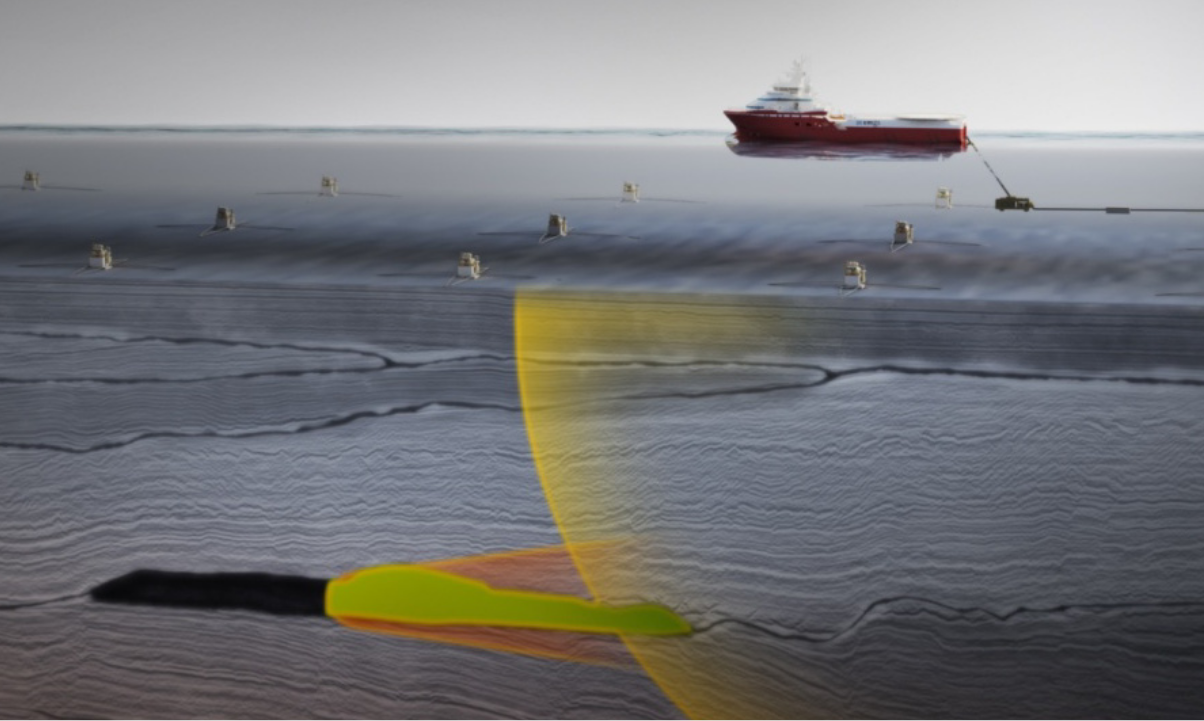
\includegraphics[width=\textwidth,height=\textheight,keepaspectratio]{10000000000004B4000002D101BC1A4D.png}
	\end{figure}
\end{frame}

% =============================================================================

\begin{frame}
	\MakeTitle{Математическая модель}
	\textbf{Уравнение Гельмгольца:}
	\begin{equation}
		\nabla \times ( \mu^{-1} \nabla \times \mathbf{E} ) + k^{2} \mathbf{E} = - i \omega \mathbf{J} , \text{~~~} k^{2} = i \omega \sigma - \omega^{2} \varepsilon \label{eq:helmholtz}
	\end{equation}

	\begin{small}
	$\mathbf{E}$~--~напряжённость электрического поля~(В/м), \\
	$\sigma$~--~электрическая проводимость~(См/м), \\
	$\varepsilon = \varepsilon_r \varepsilon_0$~--~диэлектрическая проницаемость~(Ф/м), \\
	$\mu = \mu_r \mu_0$~--~магнитная проницаемость~(Гн/м), \\
	$\mathbf{J}$~--~плотность стороннего электрического тока~(А/м${}^2$).
	\end{small}
%
	\newline\newline
	\textbf{Краевые условия:}
	\begin{equation}
		\left. \mathbf{E} \times \mathbf{n} \right | _{ S_1 } = {\mathbf{E}} ^g , \label{eq:bound1}
	\end{equation}
	\begin{equation}
		\left. \sigma \mathbf{E} \cdot \mathbf{n} \right | _{ S_2 } = 0 . \label{eq:bound2}
	\end{equation}

\end{frame}

% =============================================================================

\begin{frame}
	\MakeTitle{Вариационная постановка}
	\textbf{Пространства:}
	\begin{equation*}
		\mathbb{H} ( \mathrm{rot}\,, \Omega ) = \lbrace \mathbf{v} \in [\mathbb{L}^{2}(\Omega)]^{3} : \nabla \times \mathbf{v} \in [\mathbb{L}^{2}(\Omega)]^{3} \rbrace , \label{eq:H_rot}
	\end{equation*}
	\begin{equation*}
		\mathbb{H}_{0}( \mathrm{rot}\,, \Omega ) = \lbrace \mathbf{v} \in \mathbb{H}(\mathrm{rot}\,, \Omega) : \left. \mathbf{v} \times \mathbf{n} \right|_{\partial \Omega} = 0  \rbrace . \label{eq:H0_rot}
	\end{equation*}
%
	\newline\newline
	\textbf{Вариационная постановка:} Найти $\mathbf{E} \in \mathbb{H}_{0}( \mathrm{rot}\,, \Omega )$, такое что $\forall \mathbf{v} \in \mathbb{H}_{0}( \mathrm{rot}\,, \Omega )$ будет выполнено:
	\begin{equation}
		\int\limits_\Omega \mu^{-1} \nabla \times \mathbf{E} \cdot \nabla \times \overline{\mathbf{v}} \,d\Omega + \int\limits_\Omega k^{2} \mathbf{E} \cdot \overline{\mathbf{v}} \,d\Omega = - \int\limits_\Omega i \omega \mathbf{J} \cdot \overline{\mathbf{v}} \,d\Omega . \label{eq:weak}
	\end{equation}
\end{frame}

% =============================================================================

\begin{frame}
	\MakeTitle{PML-слой}
	\textbf{PML-слой} $\Omega^{PML}$ является подобластью $\Omega$ со специальными коэффициентами, построенными таким образом, чтобы обеспечить полное поглощение электрического поля внутри слоя и не допустить его отражения от внутренних границ и прохождения через внешние границы слоя.\\
	\vspace{0.5em}
	Расчётные области без PML-слоя и с PML-слоем:
	\vspace{-1.25em}
	\begin{figure}[H]
		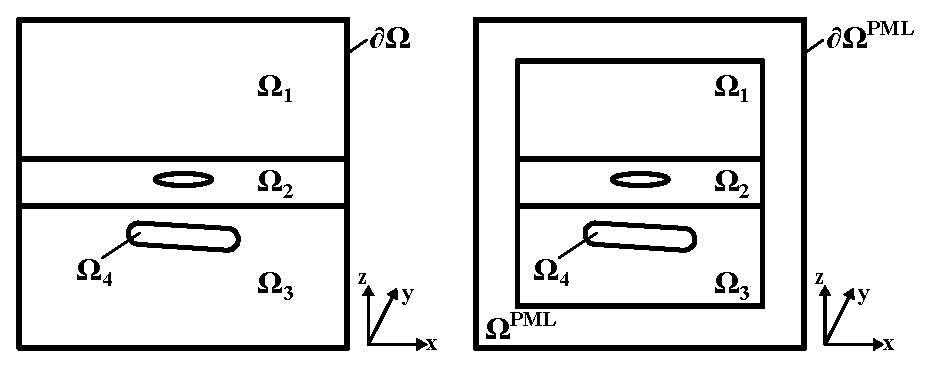
\includegraphics[width=\textwidth,height=\textheight,keepaspectratio]{area_3layers_PML.eps}
	\end{figure}
\end{frame}

% =============================================================================

\begin{frame}
	\MakeTitle{PML-слой}
	\textbf{Комплексное растяжение координат:}
	\begin{equation*}
		\tilde{x} = \int\limits_0^x s_x (t) \,dt ,
		\text{~~~~~}
		\tilde{y} = \int\limits_0^y s_y (t) \,dt ,
		\text{~~~~~}
		\tilde{z} = \int\limits_0^z s_z (t) \,dt ,
	\end{equation*}
	\begin{equation*}
		\begin{cases}
		\displaystyle
		s_j(\tau) = 1 \text{~~--~вне PML-слоя,} \\
		\displaystyle
		s_j(\tau) = 1 + \chi \left( \frac{d(\tau)}{\delta} \right)^m , \text{~~} m \geq 1 \text{~~--~внутри PML-слоя,}
		\label{eq:pml_s}
		\end{cases}
	\end{equation*}
	где $d(\tau)$ -- расстояние в $j$-м направлении от внутренней границы PML-слоя, $\delta$ -- толщина PML-слоя, $\chi$ -- некоторое комплексное число, причём $\Re(\chi) \ge 0$, $\Im(\chi) \ge 0$.
\end{frame}

% =============================================================================

\begin{frame}
	\MakeTitle{Вариационная постановка с PML-слоем}
	\textbf{Оператор $\nabla$ в новых координатах:}
	\begin{equation*}
		\tilde{\nabla} = \left[ \frac{1}{s_x} \frac{\partial}{\partial x} \,, \frac{1}{s_y} \frac{\partial}{\partial y} \,, \frac{1}{s_z} \frac{\partial}{\partial z} \right] .
	\end{equation*}

	\textbf{Вариационная постановка:}\newline Найти $\mathbf{E} \in \mathbb{H}_{0}( \mathrm{rot}\,, \widehat{\Omega} = \Omega \setminus {\Omega^{PML}} )$ и  $\tilde{\mathbf{E}} \in \mathbb{H}_{0}( \mathrm{rot}\,, {\Omega^{PML}} )$, такие что $\forall \mathbf{v} \in \mathbb{H}_{0}( \mathrm{rot}\,, \widehat{\Omega} )$ и $\forall \tilde{\mathbf{v}} \in \mathbb{H}_{0}( \mathrm{rot}\,, {\Omega^{PML}} )$ будет выполнено:
\begin{equation*}
	\begin{cases}
		\displaystyle
		\int\limits_{\widehat{\Omega}} \mu^{-1} \nabla \times \mathbf{E} \cdot \nabla \times \overline{\mathbf{v}} \,d\widehat{\Omega} + \int\limits_{\widehat{\Omega}} k^{2} \mathbf{E} \cdot \overline{\mathbf{v}} \,d\widehat{\Omega} = - \int\limits_{\widehat{\Omega}} i \omega \mathbf{J} \cdot \overline{\mathbf{v}} \,d\widehat{\Omega} \\
		\displaystyle
		\int\limits_{{\Omega^{PML}}} \mu^{-1} \tilde{\nabla} \times \tilde{\mathbf{E}} \cdot \tilde{\nabla} \times \tilde{\overline{\mathbf{v}}} \,d{\Omega^{PML}} + \int\limits_{{\Omega^{PML}}} k^{2} \tilde{\mathbf{E}} \cdot \tilde{\overline{\mathbf{v}}} \,d{\Omega^{PML}} = 0 . \\
	\end{cases}
\end{equation*}
\end{frame}

% =============================================================================

\begin{frame}
	\MakeTitle{Исследование влияния слоя воздуха}
	\textbf{Описание расчётной области}
	\begin{columns}[t,totalwidth=\linewidth]
		\begin{column}{.5\linewidth}
			\vspace{-3em}
			\begin{figure}[ht]
				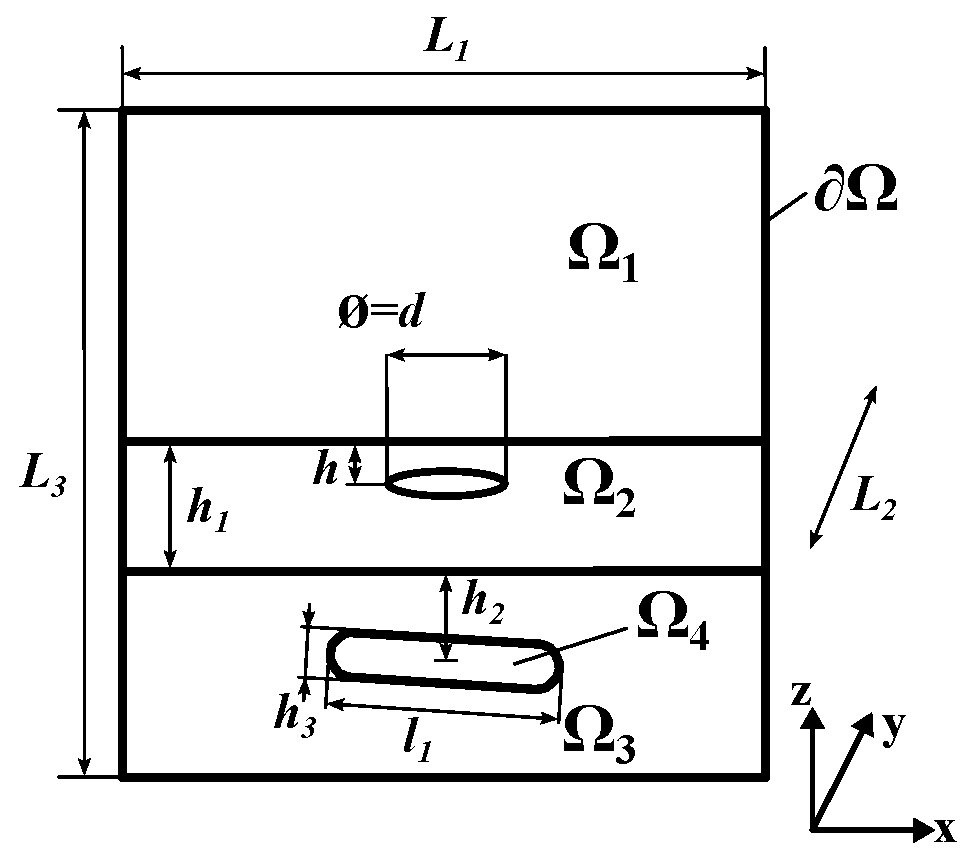
\includegraphics[width=1.1\textwidth,height=1.1\textheight,keepaspectratio]{area_3layers_shift_3.eps}
			\end{figure}
		\end{column}
		\begin{column}{.04\linewidth}
		\end{column}
		\begin{column}{.8\linewidth}
			\\
			\begin{small}
			$\Omega_1$ -- воздух ($\sigma=10^{-6}$ См/м); \\
			$\Omega_2$ -- морская вода ($\sigma=3.3$ См/м); \\
			$\Omega_3$ -- грунт ($\sigma=0.2$ См/м); \\
			$\Omega_4$ -- углеводороды ($\sigma=10^{-2}$~См/м); \\
			$L_1 = L_2 = L_3 = 6000$~м; \\
			$h_1=600$~м; $h_2=135$~м; \\
			$h_3=75$~м; $l_1=400$~м; \\
			$d=100$~м; $\nu=1$~Гц. \\
			$h$ варьируется в ходе исследования.
			\end{small}
		\end{column}
	\end{columns}
\end{frame}

% =============================================================================

\begin{frame}
	\MakeTitle{Исследование влияния слоя воздуха}
	\textbf{Относительная разность решений при изменении глубины петли $h$:}
	\begin{small}
	\begin{table}[ht]
		\begin{tabularx}{\textwidth}{|C{2.89}|C{0.73}|C{0.73}|C{0.73}|C{0.73}|C{0.73}|C{0.73}|C{0.73}|}
			\hline Глубина петли & 5 & 10 & 50 & 100 & 200 & 300 & 400 \\
			\hline $\displaystyle \frac{\| \mathbf{E}^{air} - \mathbf{E}^{noair} \|_{\mathbb{L}^2}}{\| \mathbf{E}^{air} \|_{\mathbb{L}^2}}$ & 0.44 & 0.40 & 0.24 & 0.14 & 0.07 & 0.04 & 0.02 \\
			\hline
		\end{tabularx}
	\end{table}
	\end{small}
	\vspace{-1em}
	\begin{figure}[ht]
		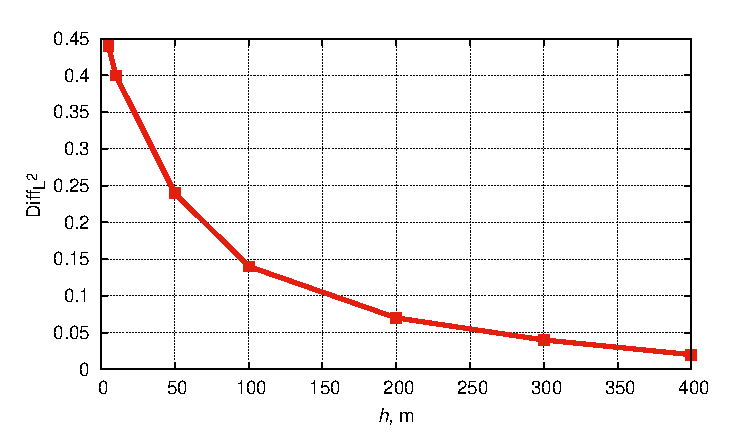
\includegraphics[scale=0.7]{presentation.eps}
	\label{fig:res1:graph}
	\end{figure}
\end{frame}

% =============================================================================

\begin{frame}
	\MakeTitle{Исследование влияния слоя воздуха}
	\textbf{$\Re(\mathbf{E}_y)$ по линии $y=0$, $z=-610$:}
	\begin{columns}[t,totalwidth=\linewidth]
		\begin{column}{.5\linewidth}
			\vspace{-1.7em}
			\begin{center}
			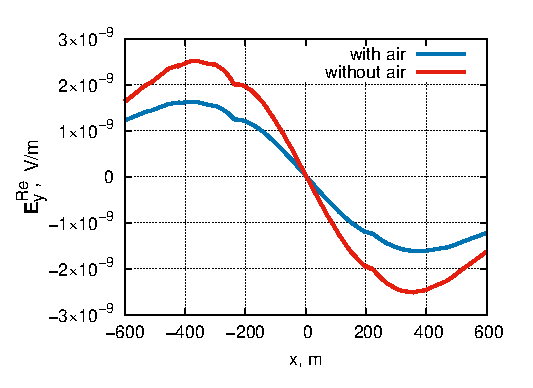
\includegraphics[width=\textwidth,height=0.4\textheight,keepaspectratio]{deep_-5.eps} \\
			\vspace{-0.1em}
			\tiny{$h=5$~м} \\
			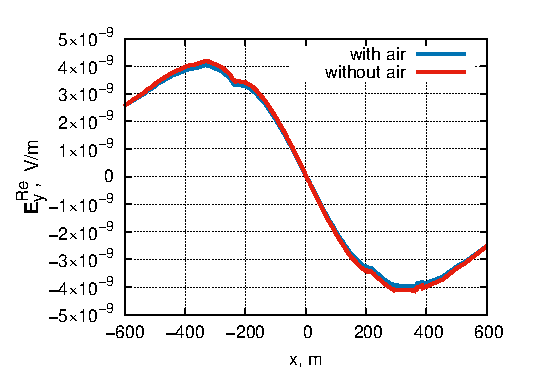
\includegraphics[width=\textwidth,height=0.4\textheight,keepaspectratio]{deep_-200.eps} \\
			\vspace{-0.1em}
			\tiny{$h=200$~м} \\
			\end{center}
		\end{column}
		\begin{column}{.5\linewidth}
			\vspace{-1.7em}
			\begin{center}
			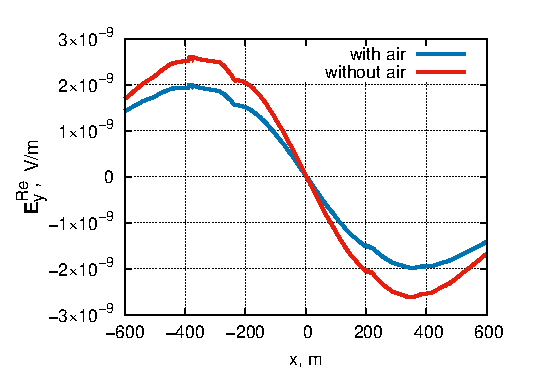
\includegraphics[width=\textwidth,height=0.4\textheight,keepaspectratio]{deep_-50.eps} \\
			\vspace{-0.1em}
			\tiny{$h=50$~м} \\
			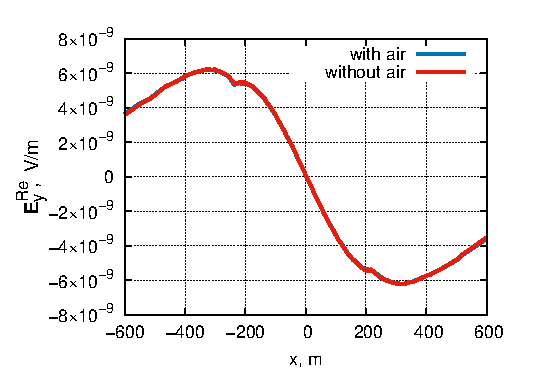
\includegraphics[width=\textwidth,height=0.4\textheight,keepaspectratio]{deep_-300.eps} \\
			\vspace{-0.1em}
			\tiny{$h=300$~м} \\
			\end{center}
		\end{column}
	\end{columns}
\end{frame}

% =============================================================================

\begin{frame}
	\MakeTitle{Исследование эффективности PML-слоя}
	\textbf{Описание расчётной области}
	\begin{columns}[t,totalwidth=\linewidth]
		\begin{column}{.5\linewidth}
			\vspace{-3em}
			\begin{figure}[ht]
				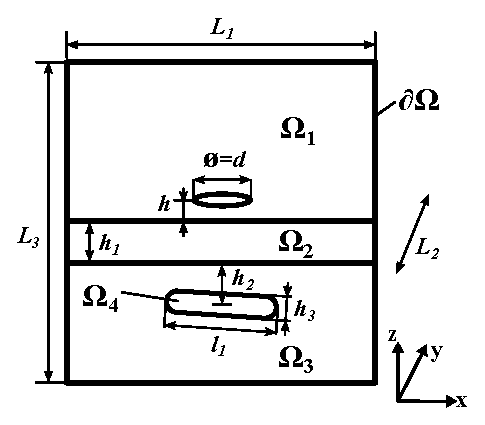
\includegraphics[width=1.1\textwidth,height=1.1\textheight,keepaspectratio]{area_3layers_3.eps}
			\end{figure}
		\end{column}
		\begin{column}{.04\linewidth}
		\end{column}
		\begin{column}{.8\linewidth}
			\\
			\begin{small}
			$\Omega_1$ -- воздух ($\sigma=10^{-6}$ См/м); \\
			$\Omega_2$ -- морская вода ($\sigma=3.3$ См/м); \\
			$\Omega_3$ -- грунт ($\sigma=0.2$ См/м); \\
			$\Omega_4$ -- углеводороды ($\sigma=10^{-2}$~См/м); \\
			$L_1 = L_2 = L_3 = 6000$~м; \\
			$h_1=300$~м; $h_2=100$~м; \\
			$h_3=100$~м; $l_1=400$~м; \\
			$d=100$~м; $\nu=1$~Гц; \\
			$h=5$~м.
			\end{small}
		\end{column}
	\end{columns}
\end{frame}

% =============================================================================

\begin{frame}
	\MakeTitle{Исследование эффективности PML-слоя}

	\textbf{Варьирование коэффициентов растяжения:}
	\vspace{0.5em}
	\fontsize{9}{12}\selectfont {
	\begin{tabularx}{\textwidth}{|N{0.7}|N{0.7}|N{0.7}|N{0.7}|N{0.7}|N{0.7}|C{2.9}|C{0.95}|C{0.95}|}
		\hline $\Re(\chi)$ в~$\Omega_1$ & $\Im(\chi)$ в~$\Omega_1$ & $\Re(\chi)$ в~$\Omega_2$ & $\Im(\chi)$ в~$\Omega_2$ & $\Re(\chi)$ в~$\Omega_3$ & $\Im(\chi)$ в~$\Omega_3$ & \raisebox{-0.8em}{$\smash{\displaystyle \frac{\lVert \Re(\mathbf{E}_y^{\text{бак}} - \mathbf{E}_y^{\text{PML}})\rVert}{\lVert \Re(\mathbf{E}_y^{\text{бак}})\rVert}}$} & Время, бак & Время, PML \\[0.2em]
		\hline 3 & 0 & 1 & 5 & 3 & 1 & 0.106636 & \multirow{4}{*}{650} & 592 \\
		\cline{1-7}\cline{9-9} 3 & 1 & 0 & 6 & 2 & 1 & 0.0925 & & 599 \\
		\cline{1-7}\cline{9-9} 4 & 0 & 1 & 5 & 3 & 1 & 0.0947 & & 731 \\
		\cline{1-7}\cline{9-9} 4 & 1 & 0 & 6 & 2 & 1 & 0.0910 & & 591 \\
		\hline
	\end{tabularx}
	}

	\begin{columns}[t,totalwidth=1.05\linewidth]
		\hspace{-0.055\linewidth}
		\begin{column}{.52\linewidth}
	\textbf{\\Варьирование толщины PML-слоя:}
	\vspace{0.5em}
	\fontsize{9}{12}\selectfont {
	\begin{tabularx}{\textwidth}{|N{0.3}|N{2.3}|N{0.7}|N{0.7}|}
		\hline \raisebox{-0.8em}[0.8em]{$\smash{\displaystyle \delta_k}$} & \raisebox{-0.8em}[0.8em]{$\smash{\displaystyle \frac{\lVert \Re(\mathbf{E}_y^{\text{бак}} - \mathbf{E}_y^{\text{PML}})\rVert}{\lVert \Re(\mathbf{E}_y^{\text{бак}})\rVert}}$} & Время, бак & Время, PML \\[0.2em]
		\hline 80 & 0.1199 & 673 & 1289 \\
		\hline 100 & 0.0910 & 650 & 591 \\
		\hline 120 & 0.0784 & 609 & 1142 \\
		\hline
	\end{tabularx}
	}
		\end{column}

		\begin{column}{.52\linewidth}
	\textbf{Варьирование размера области, на границе которой вводится PML-слой:}
	\vspace{0.5em}
	\fontsize{9}{12}\selectfont {
	\begin{tabularx}{\textwidth}{|N{0.3}|N{2.3}|N{0.7}|N{0.7}|}
		\hline \raisebox{-0.8em}[0.8em]{$\smash{\displaystyle \l_k}$} & \raisebox{-0.8em}[0.8em]{$\smash{\displaystyle \frac{\lVert \Re(\mathbf{E}_y^{\text{бак}} - \mathbf{E}_y^{\text{PML}})\rVert}{\lVert \Re(\mathbf{E}_y^{\text{бак}})\rVert}}$} & Время, бак & Время, PML \\[0.2em]
		\hline 500 & 0.187456 & 628 & 587 \\
		\hline 600 & 0.0909998 & 650 & 591 \\
		\hline 800 & 0.0440642 & 718 & 658 \\
		\hline
	\end{tabularx}
	}
		\end{column}
	\end{columns}
\end{frame}

% =============================================================================

\begin{frame}
	\MakeTitle{Исследование эффективности PML-слоя}
	\textbf{Картины электрического поля $\Re(\mathbf{E}_y)$ при параметрах $\chi_{\Omega_1} = (4, 0)$, $\chi_{\Omega_2} = (1, 6)$, $\chi_{\Omega_2} = (3, 2)$ $m=3$, $l_k = 600$~м и $\delta_k = 100$~м в сечении плоскостью $y=0$:}
	\begin{columns}[t,totalwidth=\linewidth]
		\hspace{-0.07\linewidth}
		\begin{column}{.5\linewidth}
			\vspace{-2.75em}
			\begin{figure}[H]
				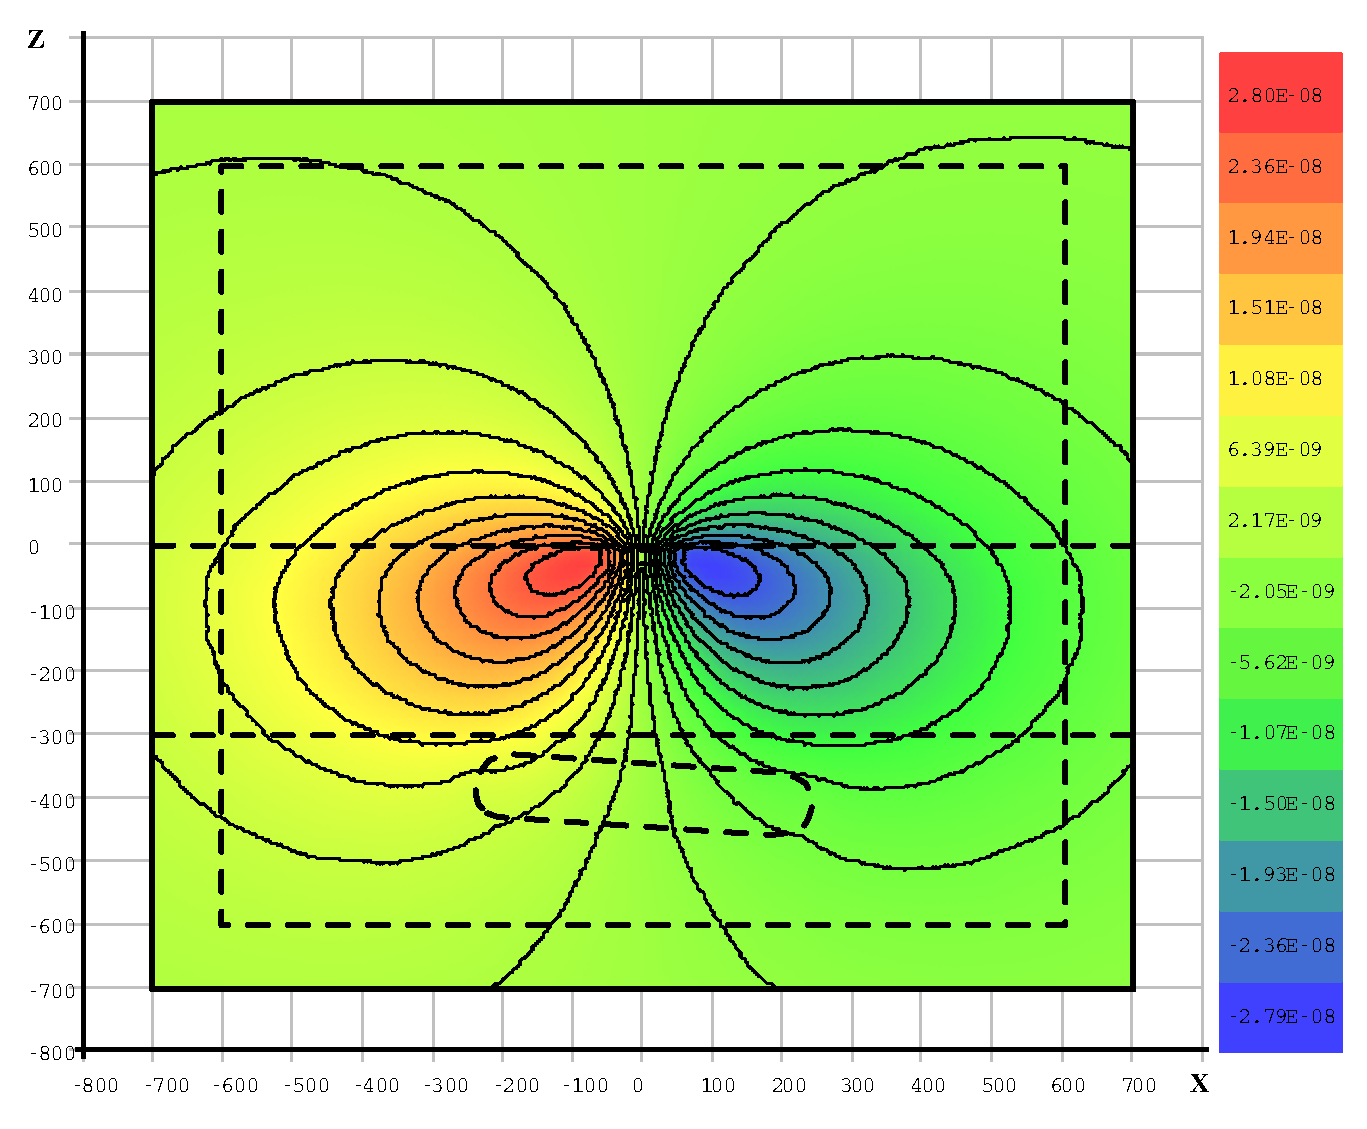
\includegraphics[width=1.1\textwidth,height=1.1\textheight,keepaspectratio]{airloop_std_y=0_EyR.eps}
			\end{figure}
			\begin{center}
				\vspace{-1em}
				\tiny{Решение с <<большим баком>>}
			\end{center}
		\end{column}
		\begin{column}{.5\linewidth}
			\vspace{-2.75em}
			\begin{figure}[H]
				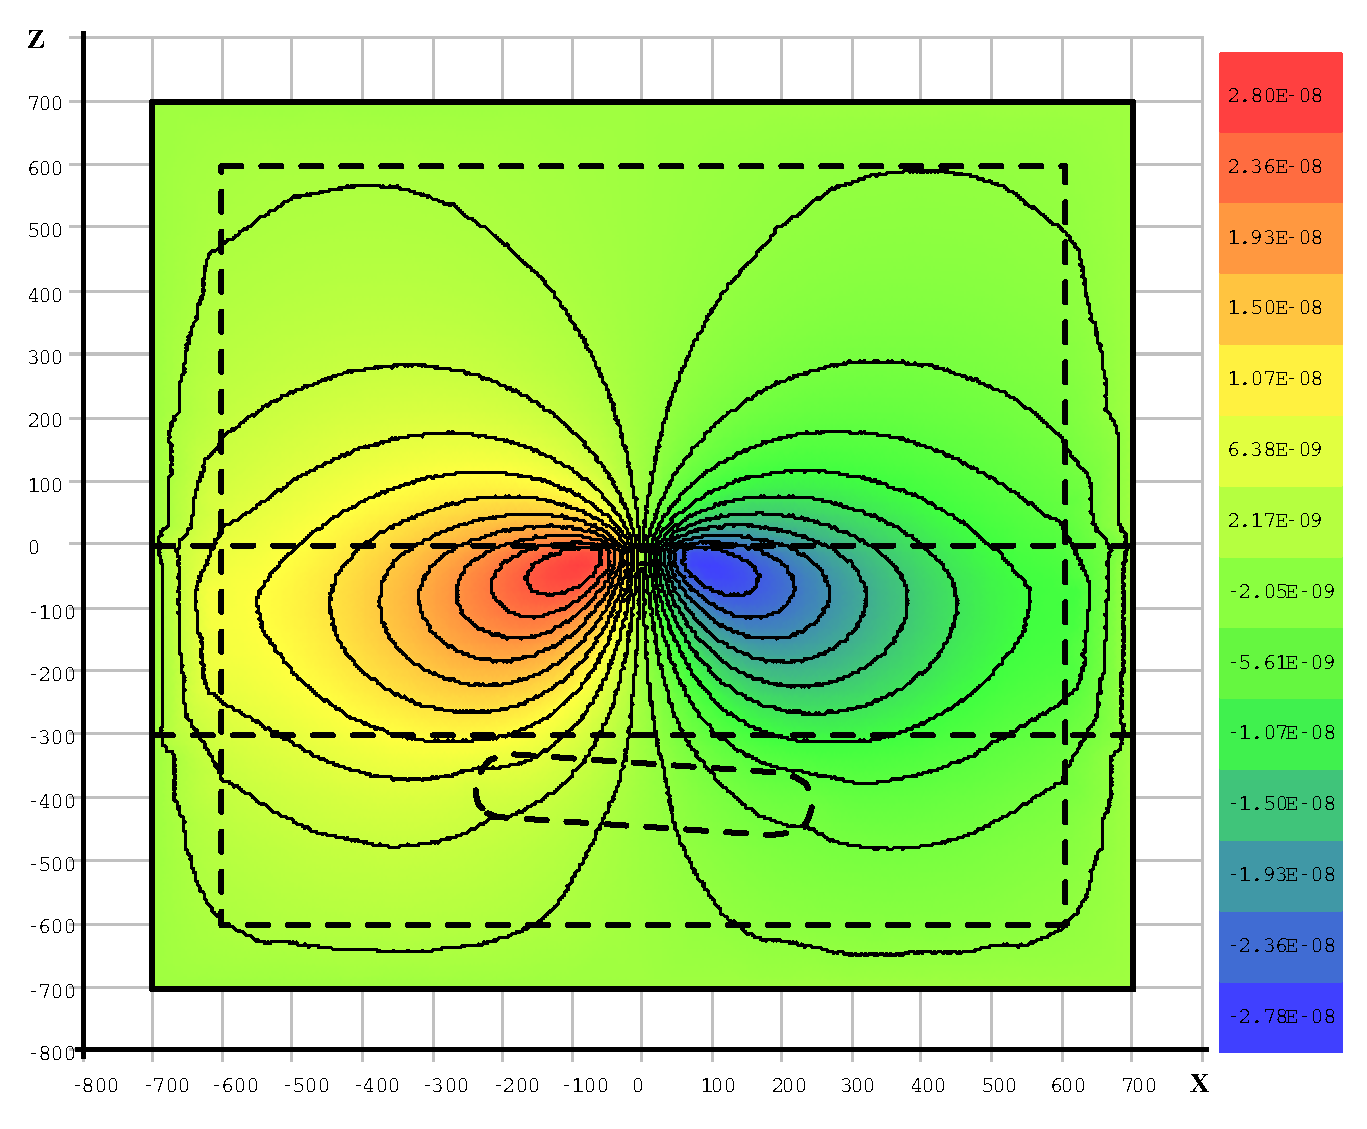
\includegraphics[width=1.1\textwidth,height=1.1\textheight,keepaspectratio]{airloop_pml_y=0_EyR.eps}
			\end{figure}
			\begin{center}
				\vspace{-1em}
				\tiny{Решение с PML-слоем}
			\end{center}
		\end{column}
	\end{columns}
\end{frame}

% =============================================================================

\begin{frame}
	\MakeTitle{Задача, приближенная к реальной}
	\textbf{Описание расчётной области}
	\begin{columns}[t,totalwidth=\linewidth]
		\hspace{-0.07\linewidth}
		\begin{column}{.5\linewidth}
			\vspace{-3em}
			\begin{figure}[ht]
				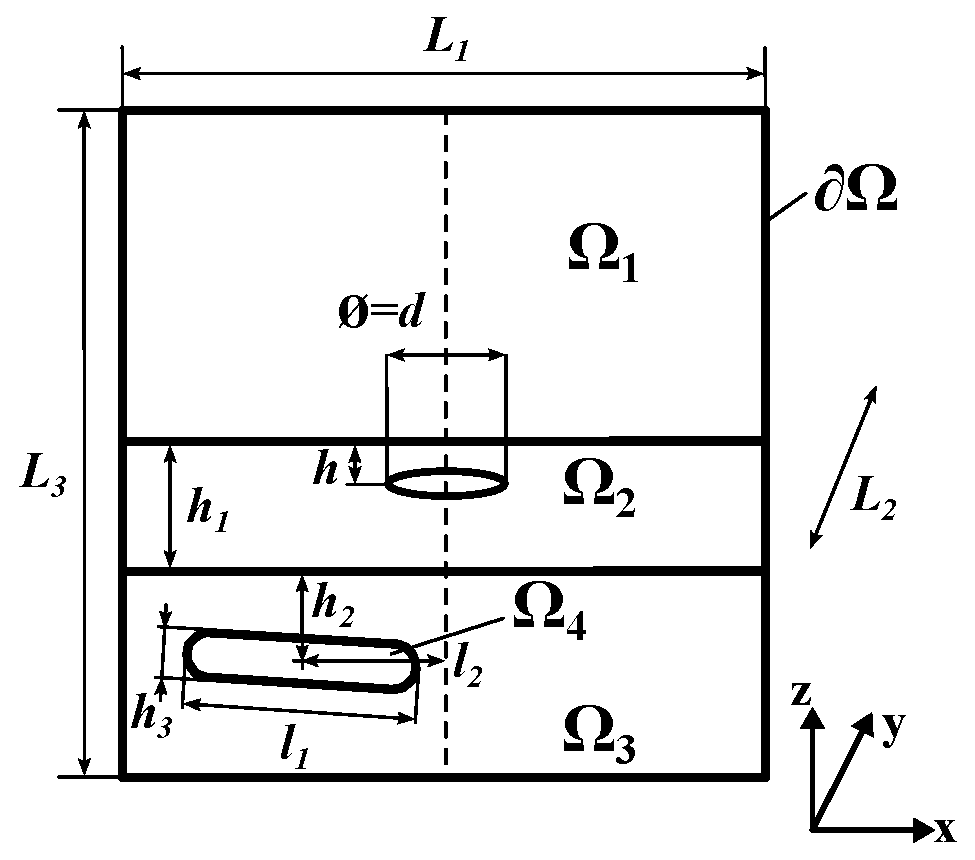
\includegraphics[width=1.1\textwidth,height=1.1\textheight,keepaspectratio]{area_3layers_shift_3_waterloop.eps}
			\end{figure}
		\end{column}
		\begin{column}{.04\linewidth}
		\end{column}
		\begin{column}{.8\linewidth}
			\\
			\begin{small}
			$\Omega_1$ -- воздух ($\sigma=10^{-6}$ См/м); \\
			$\Omega_2$ -- морская вода ($\sigma=3.3$ См/м); \\
			$\Omega_3$ -- грунт ($\sigma=0.2$ См/м); \\
			$\Omega_4$ -- углеводороды ($\sigma=10^{-2}$~См/м) \\
			или проводящий объект ($\sigma=10^{2}$~См/м); \\
			$L_1 = L_2 = L_3 = 6000$~м; \\
			$h_1=600$~м; $h_2=120$~м; \\
			$h_3=75$~м; $l_1=400$~м; \\
			$d=100$~м; $\nu=1$~Гц; $h=590$~м; \\
			$l_2 \in \{ -200, -100, 0 \}$.
			\end{small}
		\end{column}
	\end{columns}
\end{frame}

% =============================================================================

\begin{frame}
	\MakeTitle{Задача, приближенная к реальной}
	\textbf{Картины электрического поля $\Re(\mathbf{E}_z)$ при $l_2 = 0$ в сечении плоскостью $z=-601$:}
	\begin{columns}[t,totalwidth=\linewidth]
		\hspace{-0.07\linewidth}
		\begin{column}{.5\linewidth}
			\vspace{-2.75em}
			\begin{figure}[H]
				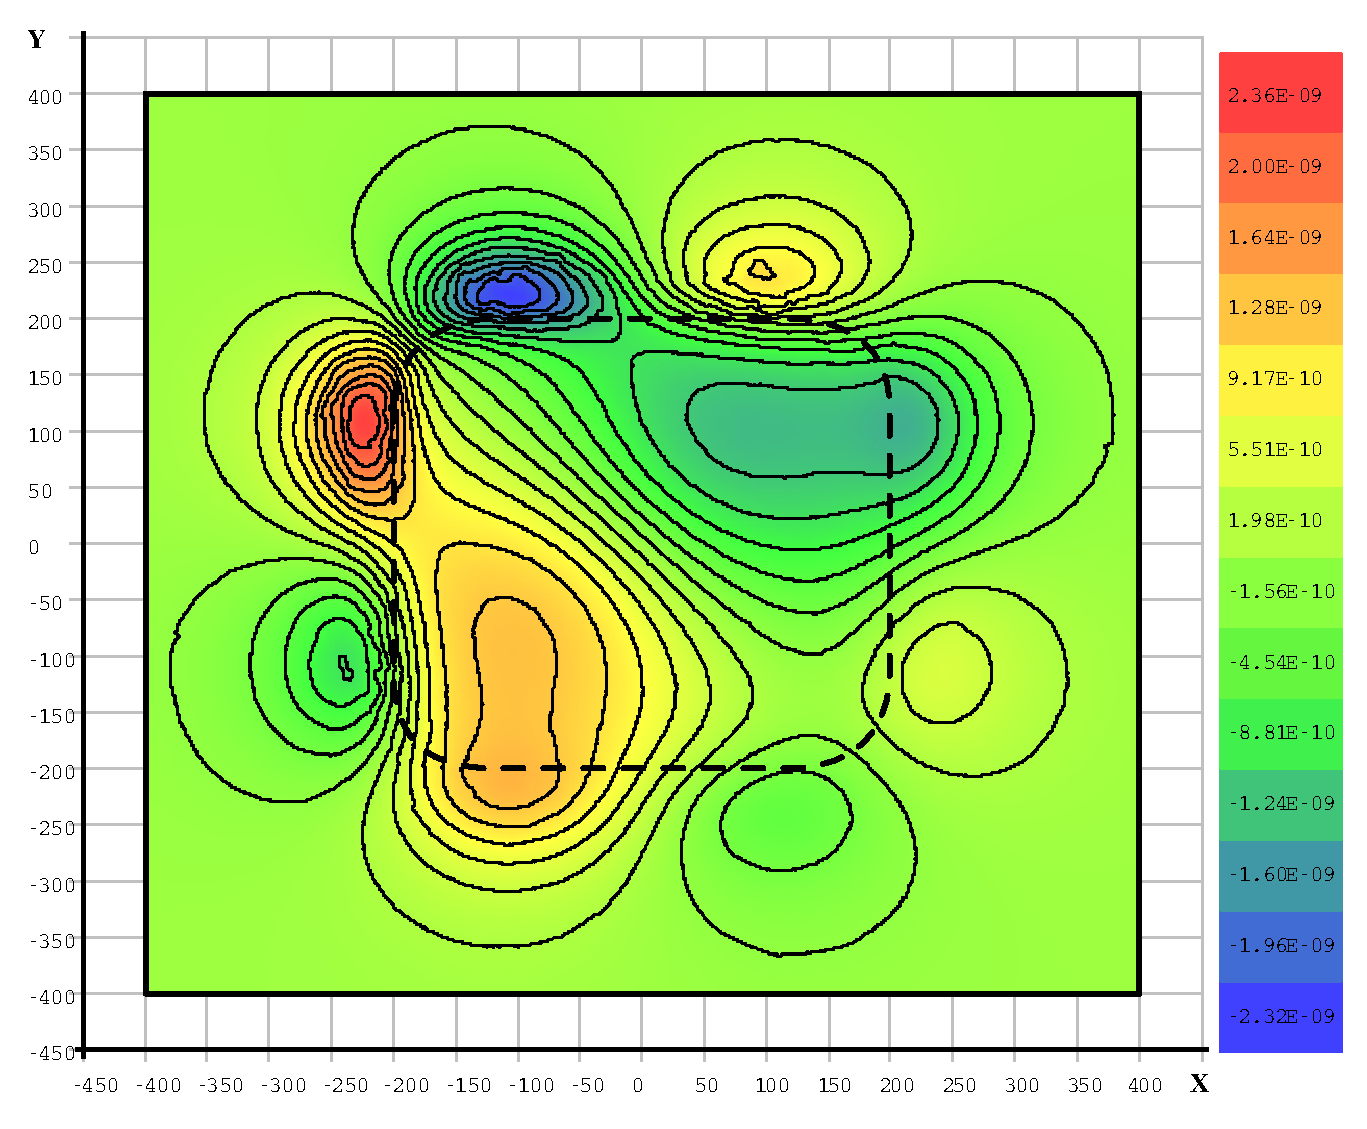
\includegraphics[width=1.1\textwidth,height=1.1\textheight,keepaspectratio]{0_no_z=-601_EzR.eps}
			\end{figure}
			\begin{center}
				\vspace{-1em}
				\tiny{Углеводороды ($\sigma = 10^{-2}$~См/м)}
			\end{center}
		\end{column}
		\begin{column}{.5\linewidth}
			\vspace{-2.75em}
			\begin{figure}[H]
				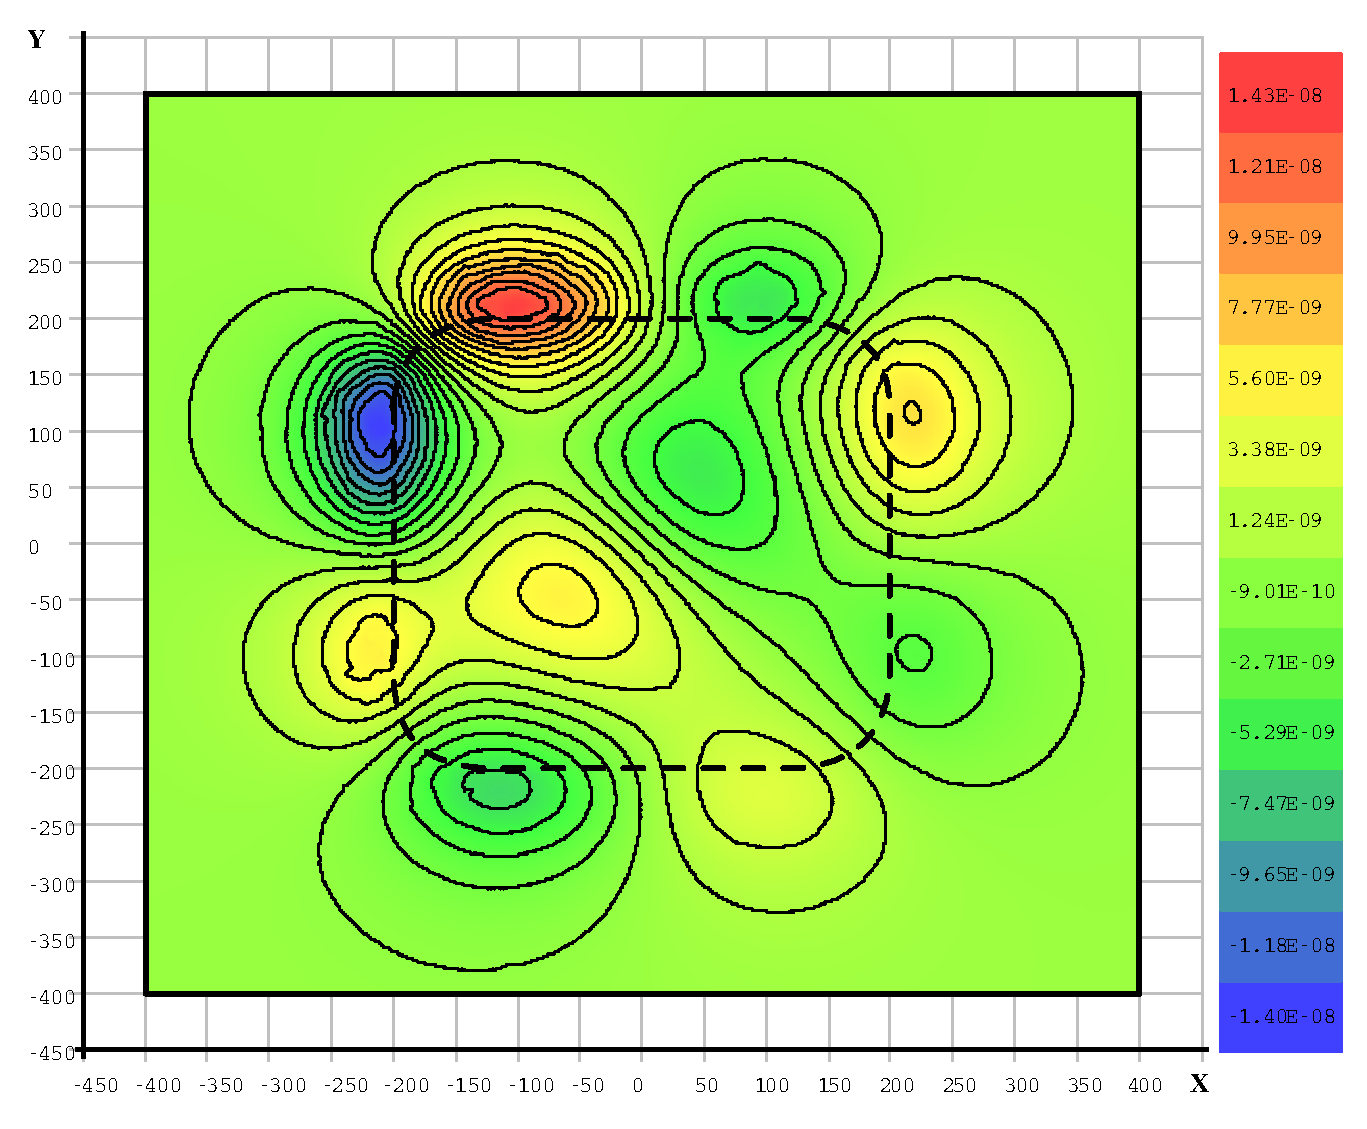
\includegraphics[width=1.1\textwidth,height=1.1\textheight,keepaspectratio]{0_yes_z=-601_EzR.eps}
			\end{figure}
			\begin{center}
				\vspace{-1em}
				\tiny{Проводящий объект ($\sigma = 10^{2}$~См/м)}
			\end{center}
		\end{column}
	\end{columns}
\end{frame}

% =============================================================================

\begin{frame}
	\MakeTitle{Задача, приближенная к реальной}
	\textbf{Картины электрического поля $\Re(\mathbf{E}_z)$ при $l_2 = -100$~м в сечении плоскостью $z=-601$:}
	\begin{columns}[t,totalwidth=\linewidth]
		\hspace{-0.07\linewidth}
		\begin{column}{.5\linewidth}
			\vspace{-2.75em}
			\begin{figure}[H]
				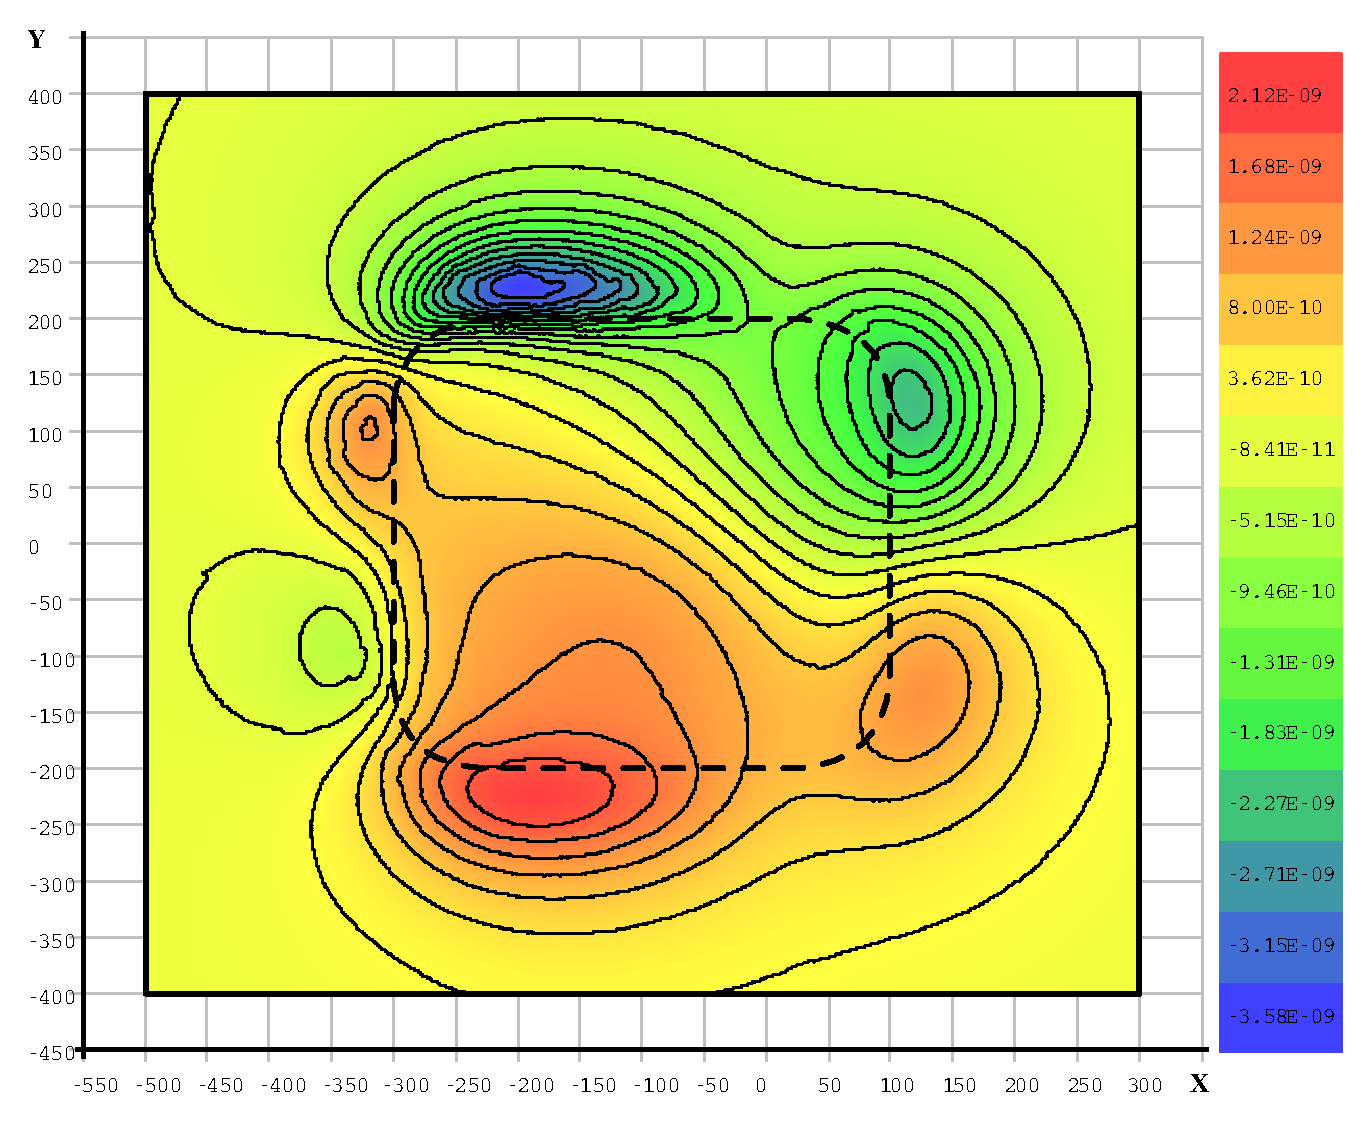
\includegraphics[width=1.1\textwidth,height=1.1\textheight,keepaspectratio]{100_no_z=-601_EzR.eps}
			\end{figure}
			\begin{center}
				\vspace{-1em}
				\tiny{Углеводороды ($\sigma = 10^{-2}$~См/м)}
			\end{center}
		\end{column}
		\begin{column}{.5\linewidth}
			\vspace{-2.75em}
			\begin{figure}[H]
				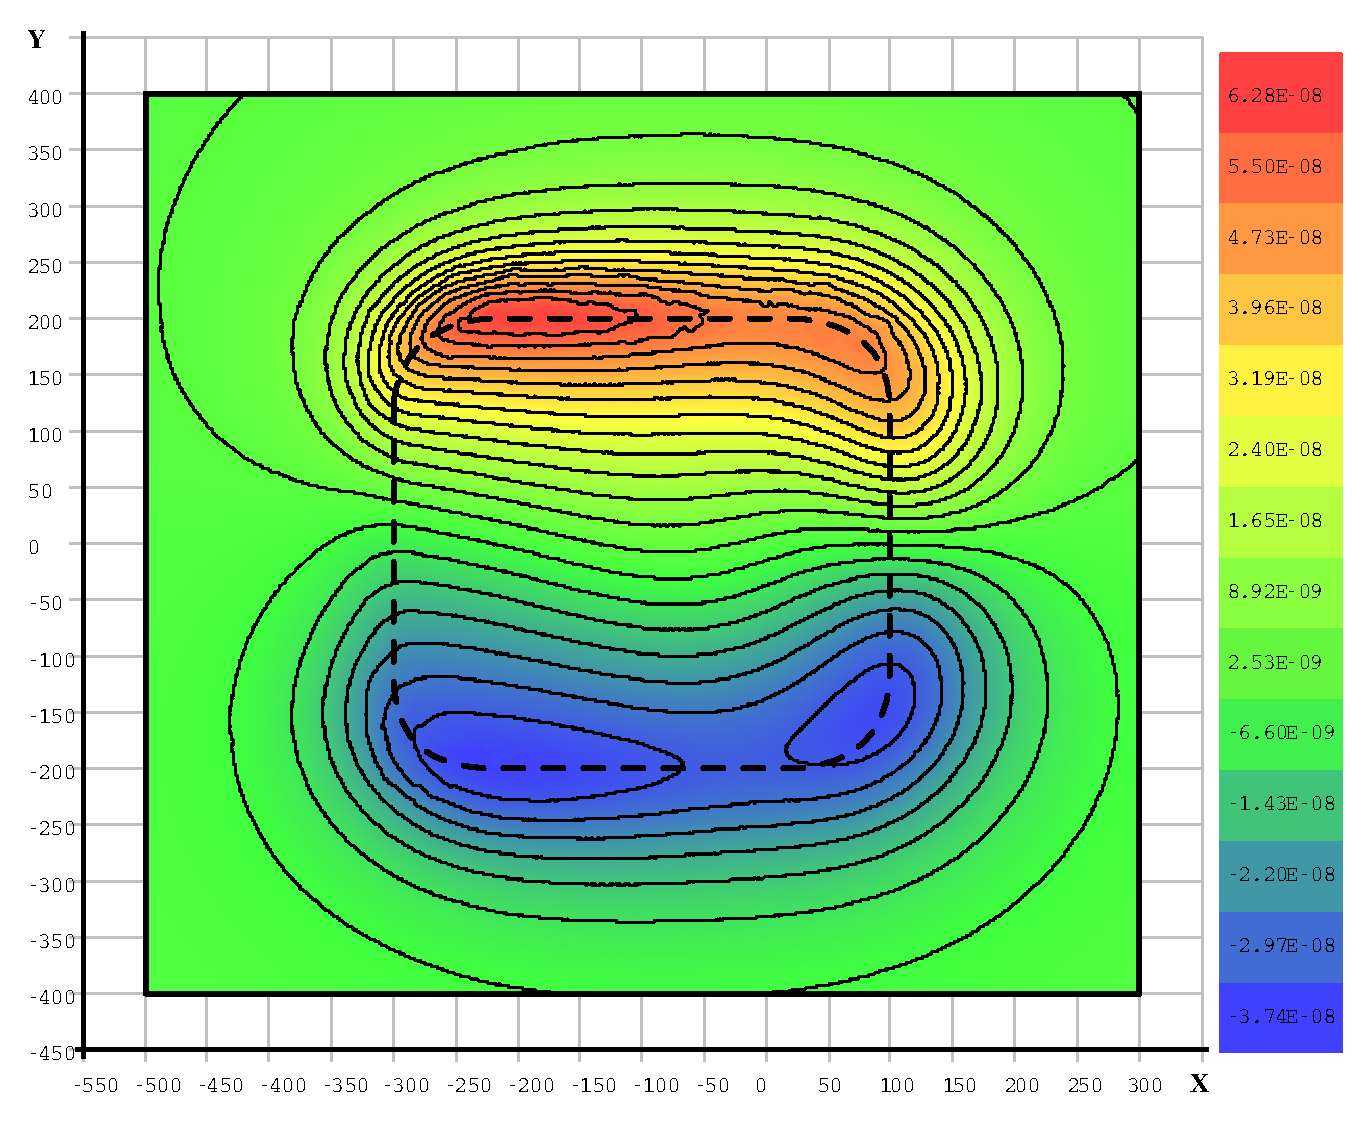
\includegraphics[width=1.1\textwidth,height=1.1\textheight,keepaspectratio]{100_yes_z=-601_EzR.eps}
			\end{figure}
			\begin{center}
				\vspace{-1em}
				\tiny{Проводящий объект ($\sigma = 10^{2}$~См/м)}
			\end{center}
		\end{column}
	\end{columns}
\end{frame}

% =============================================================================

\begin{frame}
	\MakeTitle{Задача, приближенная к реальной}
	\textbf{Картины электрического поля $\Re(\mathbf{E}_z)$ при $l_2 = -200$~м в сечении плоскостью $z=-601$:}
	\begin{columns}[t,totalwidth=\linewidth]
		\hspace{-0.07\linewidth}
		\begin{column}{.5\linewidth}
			\vspace{-2.75em}
			\begin{figure}[H]
				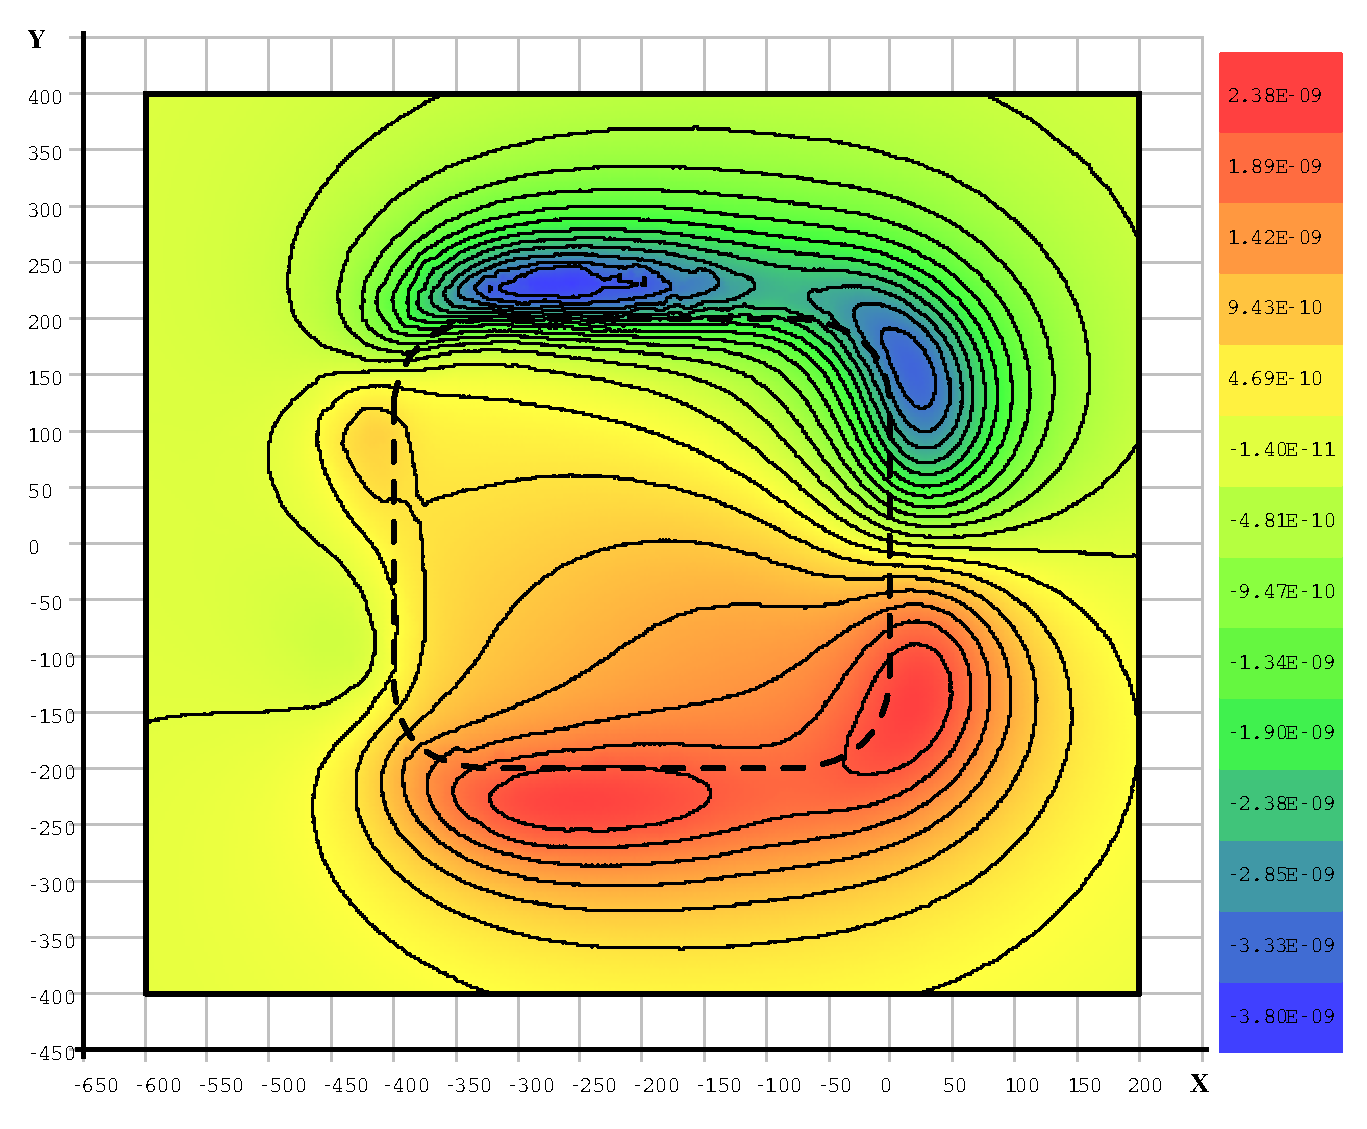
\includegraphics[width=1.1\textwidth,height=1.1\textheight,keepaspectratio]{200_no_z=-601_EzR.eps}
			\end{figure}
			\begin{center}
				\vspace{-1em}
				\tiny{Углеводороды ($\sigma = 10^{-2}$~См/м)}
			\end{center}
		\end{column}
		\begin{column}{.5\linewidth}
			\vspace{-2.75em}
			\begin{figure}[H]
				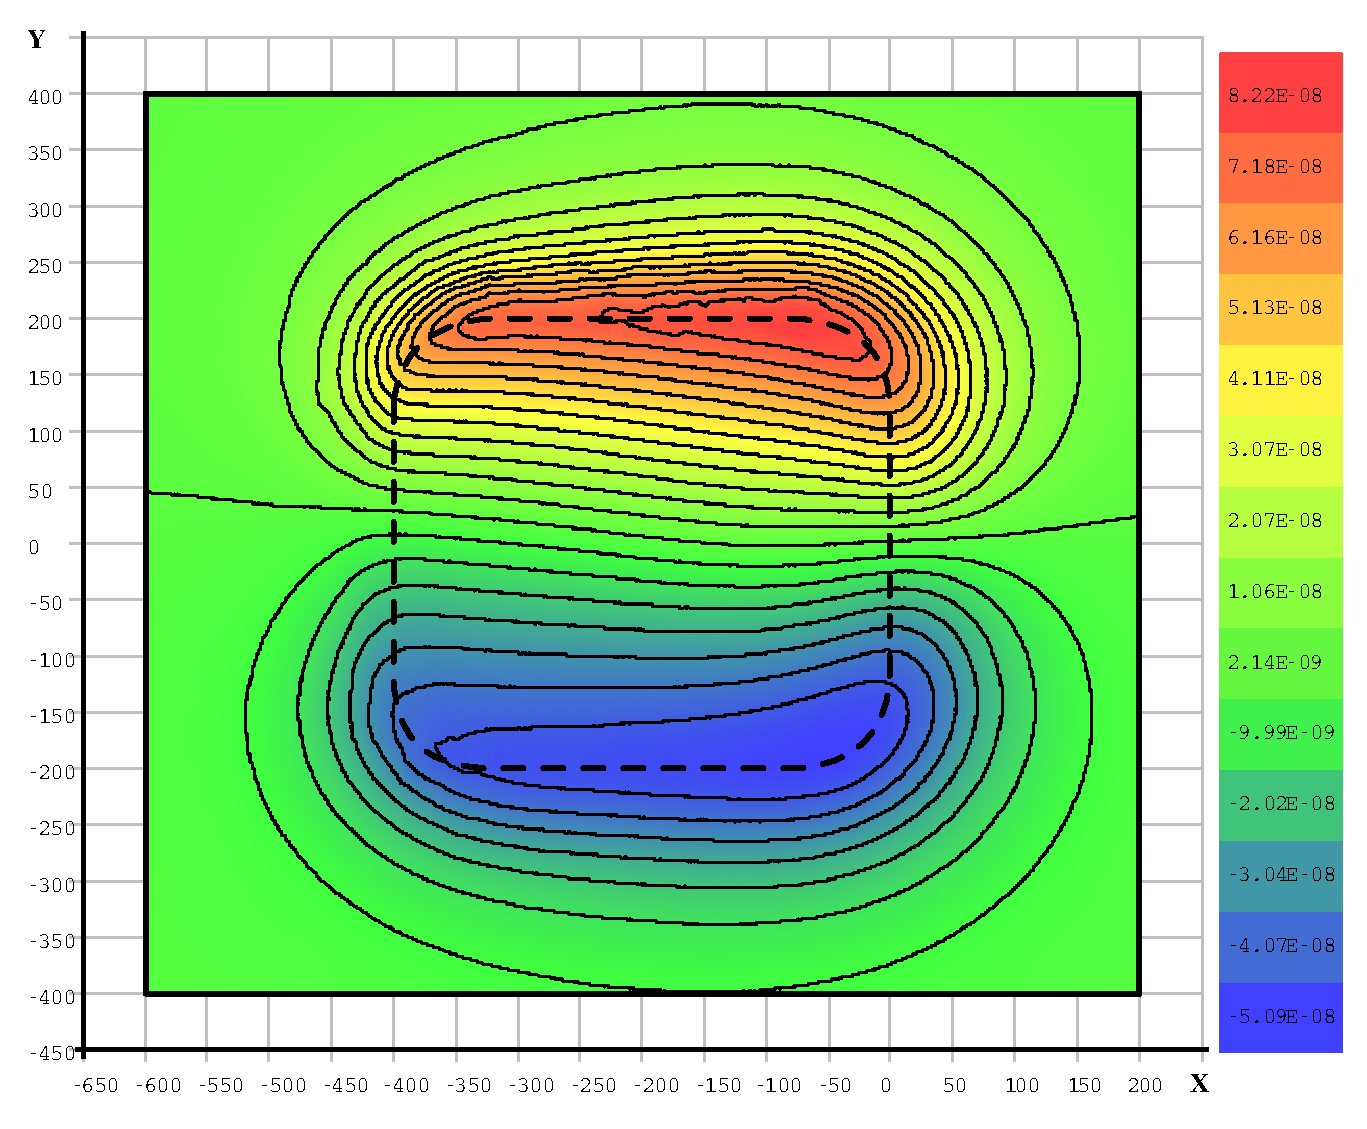
\includegraphics[width=1.1\textwidth,height=1.1\textheight,keepaspectratio]{200_yes_z=-601_EzR.eps}
			\end{figure}
			\begin{center}
				\vspace{-1em}
				\tiny{Проводящий объект ($\sigma = 10^{2}$~См/м)}
			\end{center}
		\end{column}
	\end{columns}
\end{frame}

% =============================================================================

\begin{frame}
	\MakeTitle{Заключение}
	\begin{itemize}
		\item Расчёты, в которых в область моделирования не включается воздух, допустимы только при расположении источника электромагнитного поля на большой глубине.
		\item Применение PML-слоя позволяет получить достаточно точные решения, однако его применение не приводит к резкому уменьшению размерности систем уравнений и, как следствие, к уменьшению времени решения.
		\item Проводящий объект хорошо <<виден>> на некотором расстоянии от морского дна, а непроводящий -- только вблизи дна или при небольшом заглублении приёмника в грунт. Наибольший отклик на источник электромагнитного возмущения для непроводящего объекта наблюдался в том случае, когда источник располагался со смещением от центра симметрии объекта.
	\end{itemize}
%
%	В работе были реализованы алгоритмы на базе векторного метода конечных элементов. Эти алгоритмы были положены в основу программного комплекса, который позволяет моделировать электромагнитные поля в областях разнообразной структуры. С помощью этого программного комплекса были решены модельные задачи морской геоэлектрики на низких частотах, проведены исследования возможности сокращения области моделирования без внесения дополнительных погрешностей.
%
%	На основании исследований были сделаны выводы, что расчёты, в которых в область моделирования не включается воздух, допустимы только при расположении источника электромагнитного поля на большой глубине, иначе, из-за неправильного учёта физических процессов, происходящих в воздухе, полученное решение будет неверным.
%
%	Применение PML-слоя позволило получить достаточно точные решения, однако его применение не привело к резкому уменьшению размерности систем уравнений и, как следствие, к уменьшению времени решения. Было выдвинуто предположение, что увеличить эффективность применения PML-слоя можно с помощью применения неконформных методов, в которых конечноэлементная сетка может содержать геометрические носители разного типа: тетраэдры и параллелепипеды.
%
%	Расчёты на модельной задаче с проводящим и непроводящим объектами показали, что проводящий объект хорошо <<виден>> на некотором расстоянии от морского дна, а непроводящий -- только вблизи дна или при небольшом заглублении приёмника в грунт. Наибольший отклик на источник электромагнитного возмущения для непроводящего объекта наблюдался в том случае, когда источник располагался со смещением от центра симметрии объекта.
\end{frame}


% =============================================================================


\end{document}

